\chapter{基于视觉文本化图像提示的开放词汇检测方法}

\section{引言}
目标检测方法通常依赖大规模标注数据\cite{redmon2016you,ren2016faster}，在稀缺场景（如长尾类别、专业领域与医学影像）中往往难以获取足够标注。因此，少样本目标检测（Few-shot Object Detection, FSOD）\cite{wang2019metadet,Qiao_2021_defrcn2}成为重要研究方向。近年来，视觉语言预训练模型（VLMs）通过海量图文对学习具有较强泛化能力的跨模态表示，这启发广大研究无监督方法的科研工作者可以“以文本提示进行零样本迁移”。然而，医学图像与专业领域的下游任务仍存在三类典型困难：其一，下游类别在预训练语料中覆盖不足；其二，文本提示的描述粒度有限，容易产生语义偏置与遗漏；其三，细粒度目标往往共享相近的文本描述，仅靠文本难以区分\cite{xu2023mqdet,du2022learning}。

目标级视觉语言模型（Object-level Vision-Language Models, OVLMs）\cite{li2022glip,dou2022fiber,liu2023groundingdino,minderer2022owlvit,ma2022hierkd}以 GLIP\cite{li2022glip} 为代表，利用 grounding 数据与多尺度/多阶段跨注意力结构建立了更强的\textbf{目标级图文对齐}，在零样本检测中显著优于 CLIP\cite{radford2021clip} 等图像级 VLM。然而，如何在\textbf{不破坏 OVLM 预训练的图文对齐}前提下，把下游任务中少量支持样本（support images）所包含的视觉语义注入到提示推理过程，仍然是一个关键难题。

\section{视觉文本化图像提示方法}
\subsection{研究问题与总体思路}
现有基于 VLM 的 FSOD 方法通常通过\textbf{微调原模型权重}或\textbf{引入额外可学习结构}来利用支持图像信息，但在少量目标域数据下，这两类做法都可能导致原有的目标--文本相似度分布发生偏移，从而损害源域对齐并削弱泛化能力。更进一步地，许多 OVLM（如 GLIP 与 GroundingDINO）本质上是\textbf{“仅支持文本提示”的模型}，由于结构设计限制，缺少对图像提示（image prompting）的原生支持\cite{li2022glip,liu2023groundingdino}。

图像提示为解决上述问题提供了一条思路：用支持图像作为提示，与文本提示一起为下游推理提供语义引导\cite{luddecke2022clipseg,xu2023mqdet}。然而，现有代表方法 MQ-Det\cite{xu2023mqdet} 通过在文本编码器内部额外引入可学习跨注意力模块来实现“图像调制文本”，它主要对现有文本 token 进行重加权，而非直接引入新的视觉信息；同时，新引入的结构也可能进一步偏置 OVLM 的预训练对齐。

基于此，本章提出 VisTex-OVLM：通过\textbf{视觉文本化（visual textualization）}将支持图像投影到 OVLM 的\textbf{文本特征空间}，把支持样本以“文本 token”的形式直接并入提示序列，从而在不修改 OVLM 主体结构的前提下实现\textbf{直接图像提示}。

\subsection{任务定义与符号说明}
在经典 FSOD 设置中，存在基类数据集 $D_b$（类别集合 $C_b$）与新类数据集 $D_n$（类别集合 $C_n$），满足 $C_b\cap C_n=\emptyset$。在新类集合中，每个类别仅提供至多 $K$ 个带框标注实例（$K$-shot）。测试阶段中，提供少量标注的图像称为支持图像（support images），待预测的图像称为查询图像（query images）。在更一般的 GFSOD 设置中，测试类别集合为 $C_b\cup C_n$，要求模型在新类上提升的同时保持基类性能。

对 OVLM 的多尺度/多阶段编码过程，记第 $i$ 个 stage 的中间视觉特征与文本特征分别为 $R^i$ 与 $P^i$，其中 $i=0,1,\ldots,L$。多尺度特征记为 $R^i=\left[R^{i,(j)}\right]_{j=0}^{M-1}$，其中 $M$ 表示尺度数。

\subsection{总体框架}
图 \ref{fig:vistex_framework} 给出了 VisTex-OVLM 的整体流程。其核心由两部分组成：\textbf{多尺度视觉文本化模块（Multi-scale Textualizing Blocks, MSTB）}与\textbf{多阶段融合策略（Multi-stage Fusion, MSF）}。二者共同将支持图像映射为一个或多个\textbf{视觉文本化 token}，并与常规文本提示 token 拼接后直接输入\textbf{冻结的} OVLM，实现无需改动主干结构的图像提示推理。

\begin{figure}[t]
  \centering
  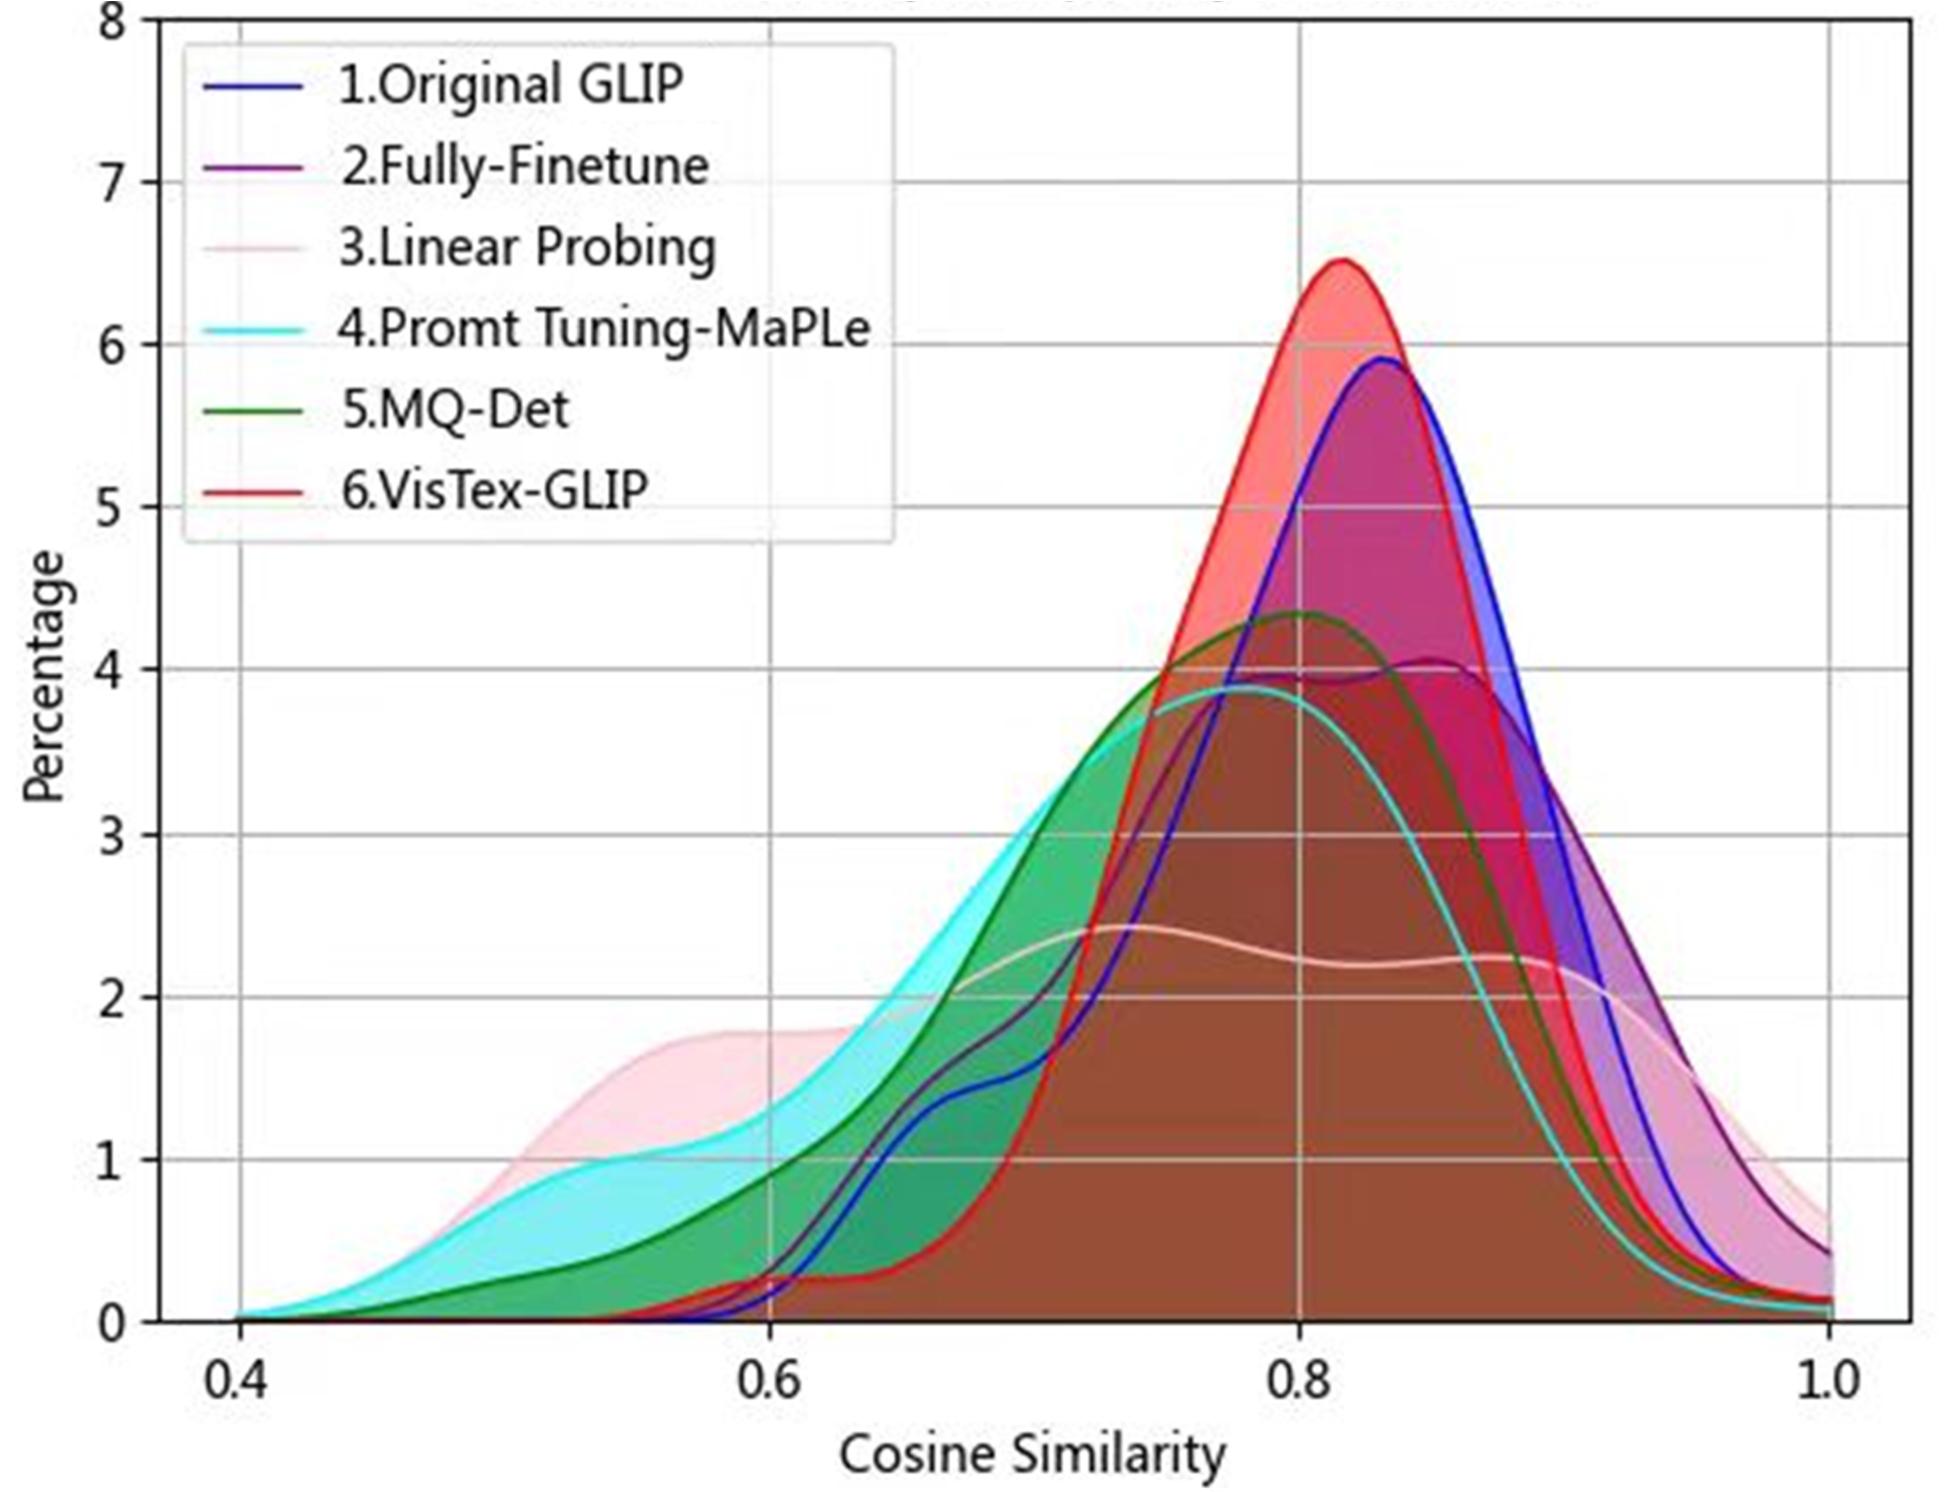
\includegraphics[width=0.96\linewidth]{chapters/PAPERS/VisTex_ICCV_ver/cosine1.png}
  \caption{目标域适配对预训练对齐的影响}
  \label{fig:vistex_cosine}
\end{figure}
图~\ref{fig:vistex_cosine} 中，在有限目标域数据下，结构或权重的修改会使源域 object--text 相似度分布发生偏移，从而部分破坏预训练对齐。


\begin{figure}[t]
  \centering
  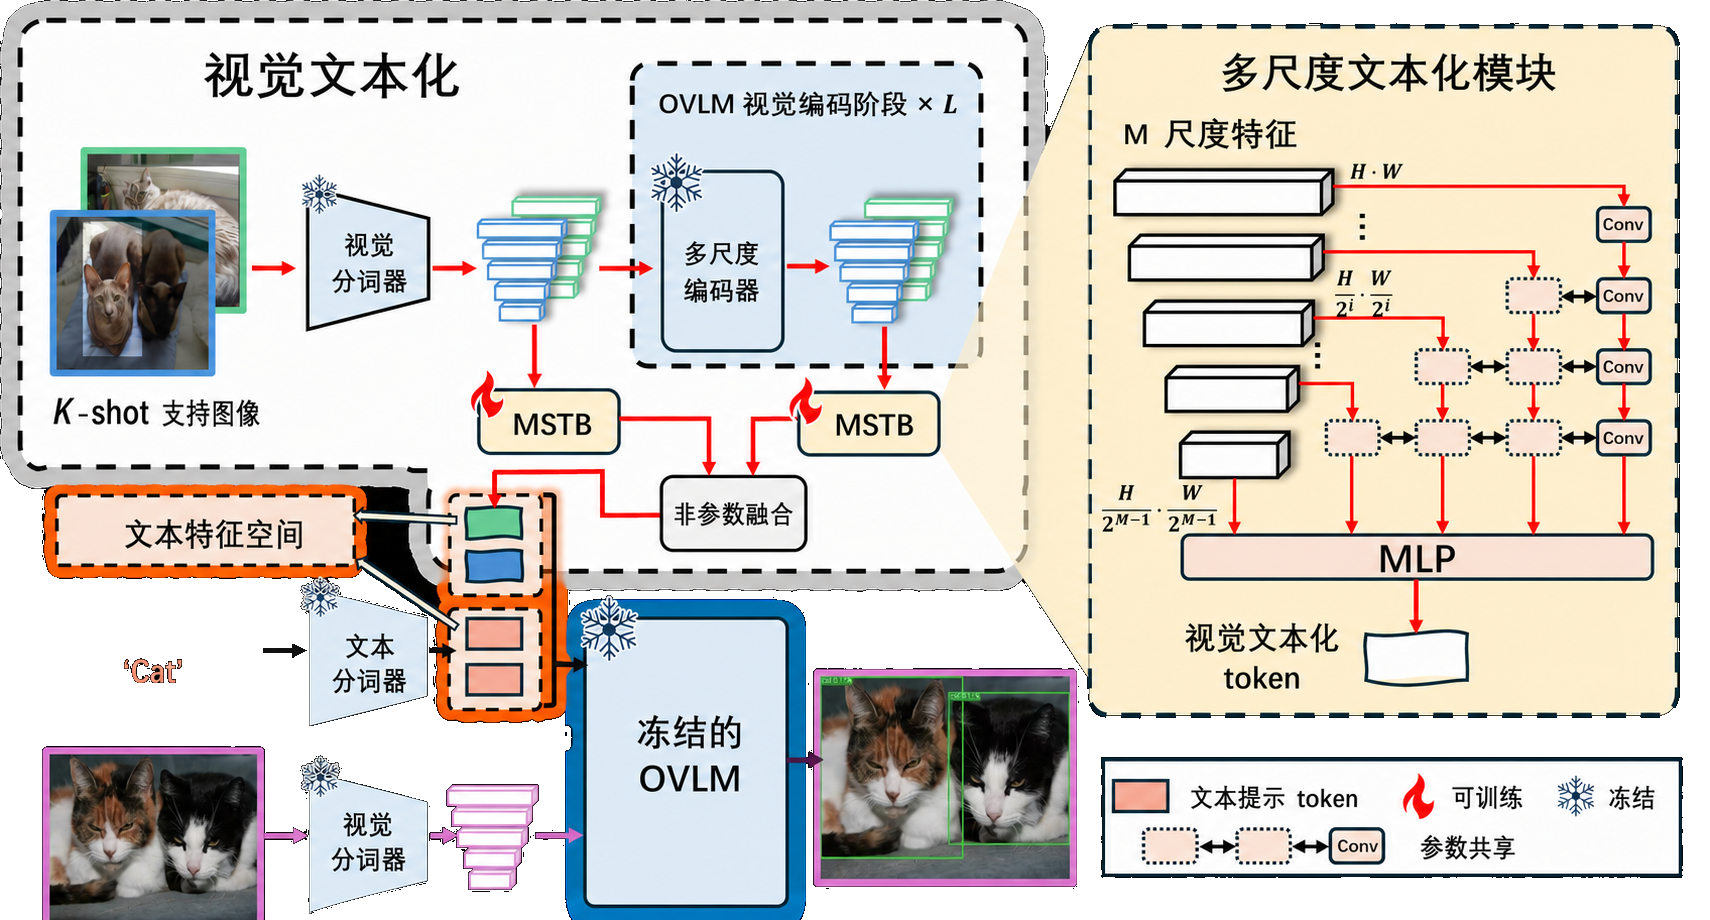
\includegraphics[width=\linewidth]{figures/figure4_2_vistex_method_white_20260817.png}
  \caption{VisTex-OVLM 总体框架}
  \label{fig:vistex_framework}
\end{figure}
图~\ref{fig:vistex_framework} 中，通过 MSTB 与 MSF 将支持图像投影到 OVLM 的文本特征空间，生成视觉文本化 token，并与文本提示共同驱动未修改的 OVLM（如 GLIP\cite{li2022glip}、GroundingDINO\cite{liu2023groundingdino}）完成少样本检测。


\subsection{图像提示工程（Image Prompt Engineering）}
由于检测属于密集预测任务，支持图像中同时包含目标、背景及其它干扰物体。为最大化利用少样本标注，本章采用图像提示工程：结合支持图像中的目标框信息，对框外区域进行模糊化处理，使得支持图像更聚焦于目标实例\cite{luddecke2022clipseg}。

\subsection{多尺度视觉文本化（MSTB）}
给定提示工程后的支持图像 $x_S$，使用冻结的 OVLM 视觉编码器提取各 stage 的多尺度特征 $R^i_S=\left[R_S^{i,(j)}\right]_{j=0}^{M-1}$。MSTB 的目标是将不同尺度的视觉特征统一聚合，并映射到文本特征维度，从而得到 stage 级的视觉文本化特征 $\widetilde{P^i_S}$。

为高效共享跨尺度知识并降低训练成本，MSTB 采用参数共享策略：对除最小尺度以外的各尺度特征使用共享的下采样卷积逐级压缩到同一空间分辨率，拼接后再用 MLP 映射到文本空间，形式化为：
\begin{equation}
\begin{aligned}
    \widetilde{R^{i,(j)}_S} = \left\{
    \begin{array}{ll}
    \left( \prod_{j}^{M-2} \operatorname{Conv}_{\text{down}}^{i,(j)}\right) \left( R^{i,(j)}_S \right), & \text{if } j \neq M-1 \\
    R^{i,(j)}_S, & \text{if } j = M-1
    \end{array}
    \right.
\end{aligned}
\label{eq:vistex_downsample}
\end{equation}
\begin{equation}
    \widetilde{R^i_S} = \left[ \widetilde{R^{i,(j)}_S} \right]_{j=0}^{M-1},
\label{eq:vistex_concat}
\end{equation}
\begin{equation}
    \widetilde{P^i_S} = \operatorname{MLP}^i \left( \widetilde{R^i_S} \right).
\label{eq:vistex_mlp}
\end{equation}

\subsection{多阶段融合（MSF）}
OVLM 的多阶段编码对应着多阶段的跨模态对齐过程。为充分利用这种对齐先验，本章进一步对各 stage 的 $\widetilde{P^i_S}$ 进行非参数融合，得到最终的视觉文本化 token $\widetilde{P_S}$：
\begin{equation}
    \widetilde{P_S} = \operatorname{MSF} \left( \{ \widetilde{P^i_S}\}_{i=0}^L \right).
\label{eq:vistex_msf}
\end{equation}
由于 MSF 采用非参数操作（如跨 stage 的 max pooling），因此在不引入额外参数的情况下即可利用 OVLM 的多阶段对齐能力。

\subsection{直接支持图像提示（Direct Image Prompting）}
得到 $\widetilde{P_S}$ 后，将其与文本提示 $t$ 经 BERT 编码得到的 token 直接拼接，构成输入 OVLM 的提示序列：
\begin{equation}
    P^0 = \left[ \operatorname{BERT}\left(t\right), \widetilde{P_S} \right].
\label{eq:vistex_prompt_1shot}
\end{equation}
对于 $K$-shot 设置，为保持每个 shot 的独立性，直接拼接多个视觉文本化 token：
\begin{equation}
    P^0 = \left[ \operatorname{BERT}\left(t\right), \widetilde{P_{S_1}}, \cdots, \widetilde{P_{S_K}} \right].
\label{eq:vistex_prompt_kshot}
\end{equation}
在训练阶段，仅更新 MSTB 的参数，OVLM 主体保持冻结；训练完成后，MSTB 可直接对新类支持样本进行视觉文本化，从而在不微调 OVLM 的条件下完成少样本检测。

\section{实验设置}
本章遵循标准 FSOD 协议\cite{wang2020frustratingly,zhang2022metaDETR1}，在 PASCAL VOC\cite{everingham2010pascalvoc} 与 MSCOCO\cite{lin2014microsoftCOCO} 上评价新类检测能力，并在 GFSOD 设置下同时考察基类保持能力。为了验证方法是否真正保留了 OVLM 的开放世界迁移优势，实验进一步覆盖 LVIS\cite{gupta2019lvis}、ODinW\cite{li2022odinw} 以及 MoNuSeg\cite{kumar2017dataset}、CoNSeP\cite{graham2019hover}、LIDC 和 DeepLesion 等医学数据集。除特别说明外，GLIP 与 GroundingDINO 主体保持冻结，训练阶段仅更新视觉文本化模块；测试时将每个支持实例独立编码为视觉文本化 token，再与类别文本提示共同输入查询分支。

\subsection{支持集抽样与提示方式}
对于少样本实验，本文通常使用 1-shot、5-shot、10-shot 和 50-shot 四种设置。这里的 shot 指每个类别从目标域训练集中选取的支持图像数量。为了计算平均值和标准差，实验通常使用 3 个随机种子生成三组不同支持集。需要强调的是，支持图像的选择必须在不同方法之间保持一致，否则方法差异可能被数据抽样差异掩盖。

在图像提示方法中，支持集有两种不同用途。第一，它可以作为目标域微调数据，用于更新模型部分参数。第二，它也可以只作为提示输入，在不更新模型权重的情况下为测试图像提供目标域上下文。前者通常可能获得更高性能，但需要额外训练成本；后者更加轻量，适合快速部署和公平比较。本文后续主表和消融实验中，需要明确区分这两类设置。

\section{实验结果与分析}
\subsection{标准少样本检测结果}
表 \ref{tab:vistex_fsod} 汇总了 MSCOCO 新类在不同 shot 数下的代表性结果。GLIP-ZS 和 GroundingDINO-ZS 不使用支持图像，因此其结果不随 shot 数变化；完全微调虽然可以利用支持样本，但在极低样本条件下容易过拟合。相比之下，VisTex-GLIP 从 1-shot 的 47.9 AP 提升到 30-shot 的 53.6 AP，VisTex-DINO 则由 48.9 AP 提升到 55.4 AP。更重要的是，在 1--5 shot 的数据极度受限区间，视觉文本化已经能够稳定超过对应的零样本和完全微调基线，说明增益并非来自大规模目标域训练，而是来自支持图像语义与预训练对齐空间的有效结合。

\begin{table}[t]
  \centering
  \caption{MSCOCO 新类少样本检测结果}
  \label{tab:vistex_fsod}
  \resizebox{\linewidth}{!}{
  \begin{tabular}{l|rrrrrr}
    \hline
    方法 & 1-shot & 2-shot & 3-shot & 5-shot & 10-shot & 30-shot \\ \hline
    GLIP-ZS & 42.9 & 42.9 & 42.9 & 42.9 & 42.9 & 42.9 \\
    GLIP-FF & 41.2 & 44.7 & 47.5 & 48.8 & 49.3 & 49.4 \\
    MQ-Det & 42.2 & 46.3 & 47.5 & 47.7 & 47.8 & 48.1 \\
    \textbf{VisTex-GLIP} & \textbf{47.9} & \textbf{51.8} & \textbf{52.2} & \textbf{52.6} & 52.7 & 53.6 \\ \hline
    GroundingDINO-ZS & 48.5 & 48.5 & 48.5 & 48.5 & 48.5 & 48.5 \\
    GroundingDINO-FF & 48.7 & 48.9 & 49.3 & 50.8 & 51.6 & 53.0 \\
    \textbf{VisTex-DINO} & \textbf{48.9} & \textbf{49.2} & \textbf{50.2} & \textbf{52.5} & \textbf{54.3} & \textbf{55.4} \\ \hline
  \end{tabular}}
\end{table}
表~\ref{tab:vistex_fsod} 中，ZS 表示零样本直接测试，FF 表示对 OVLM 进行完全微调。


\subsection{广义少样本检测与基类保持}
经典 FSOD 只报告新类性能，可能掩盖模型对基类知识的遗忘。为此，表 \ref{tab:vistex_gfsod} 同时给出总体 AP、基类 AP（bAP）和新类 AP（nAP）。VisTex-GLIP 在 10-shot 和 30-shot 下均取得最高总体 AP 与 nAP，并且 bAP 没有因新类适配而明显下降。这一现象与图 \ref{fig:vistex_cosine} 的观察一致：视觉文本化把新信息写入提示序列，而不是直接改写 OVLM 参数，因此能够在吸收支持样本信息的同时保留预训练模型原有的类别覆盖能力。

\begin{table}[t]
    \centering
    \resizebox{0.8\linewidth}{!}{
    \begin{tabular}{ccccccc}
    \hline
    \multicolumn{1}{c|}{} & \multicolumn{3}{c|}{\textbf{10-shot}} & \multicolumn{3}{c}{\textbf{30-shot}} \\ \cline{2-7} 
    \multicolumn{1}{c|}{\multirow{-2}{*}{\textbf{方法}}} & \textbf{AP} & \textbf{bAP} & \multicolumn{1}{c|}{\textbf{nAP}} & \textbf{AP} & \textbf{bAP} & \textbf{nAP} \\ \hline
    \multicolumn{7}{c}{\textbf{非 VLM 方法}} \\ \hline
    \multicolumn{1}{c|}{\textbf{DiGeo \cite{ma2023digeo}}} & 32.0 & 39.2 & \multicolumn{1}{c|}{10.3} & 33.1 & 39.4 & 14.2 \\
    \multicolumn{1}{c|}{\textbf{DE-VIT-L \cite{zhang2023devit}}} & 30.6 & 29.4 & \multicolumn{1}{c|}{34.0} & 30.6 & 29.5 & 34.0 \\ \hline
    \multicolumn{7}{c}{\textbf{VLM 方法}} \\ \hline
    \multicolumn{1}{c|}{\textbf{FM-FSOD-L \cite{Han_2024_FM-FSOD}}} & 40.0 & 44.2 & \multicolumn{1}{c|}{27.7} & 43.1 & 45.2 & 37.0 \\
    \multicolumn{1}{c|}{\textbf{MQ-Det \cite{xu2023mqdet}}} & 46.9 & \textbf{46.5} & \multicolumn{1}{c|}{47.8} & 47.3 & 46.8 & 48.1 \\
    \multicolumn{1}{c|}{\textbf{VisTex-GLIP}} & \textbf{48.1} & 46.2 & \multicolumn{1}{c|}{\textbf{52.7}} & \textbf{48.9} & \textbf{47.2} & \textbf{53.6} \\ \hline
    \end{tabular}
    }
    \caption{MSCOCO 广义少样本检测结果}
    \label{tab:vistex_gfsod}
\end{table}
表~\ref{tab:vistex_gfsod} 中，bAP/nAP 分别表示 base/novel 类别 AP。


\subsection{开放集与医学数据迁移}
为了排除“目标类别已经在预训练语料中出现”的影响，本章把在 MSCOCO 基类上训练的模型直接迁移到类别重叠较少的开放集数据。表 \ref{tab:vistex_medical} 给出了五个医学数据集的 2-shot 结果。普通少样本检测器和直接零样本 GLIP 在显著域偏移下性能较低，而 VisTex-GLIP 在 MoNuSeg、CCRCC、CoNSeP、LIDC 与 DeepLesion 上分别达到 28.9、31.5、35.7、12.2 和 11.7 AP。这一结果说明，支持图像提供的不仅是类别名称的补充，而是包含染色、形态、尺度与局部上下文的目标级视觉证据。

\begin{table}[t]
  \centering
  \caption{医学数据集开放集迁移结果}
  \label{tab:vistex_medical}
  \resizebox{\linewidth}{!}{
  \begin{tabular}{l|rrrrr}
    \hline
    方法 & MoNuSeg & CCRCC & CoNSeP & LIDC & DeepLesion \\ \hline
    Meta-DETR & 15.5 & 18.2 & 19.9 & 1.2 & 0.6 \\
    DiGeo & 18.2 & 20.4 & 22.8 & 6.1 & 2.3 \\
    DeFRCN & 16.3 & 18.8 & 20.1 & 5.2 & 2.8 \\
    MFD & 19.5 & 24.2 & 18.0 & 7.5 & 3.5 \\
    MQ-Det & 17.7 & 18.9 & 16.7 & 6.3 & 3.1 \\
    GLIP-ZS & 4.2 & 8.8 & 1.3 & 0.3 & 0.0 \\
    \textbf{VisTex-GLIP} & \textbf{28.9} & \textbf{31.5} & \textbf{35.7} & \textbf{12.2} & \textbf{11.7} \\ \hline
  \end{tabular}}
\end{table}
表~\ref{tab:vistex_medical} 中，模型在 MSCOCO 基类上训练，目标医学类别不参与主干训练。


\begin{figure}[t]
  \centering
  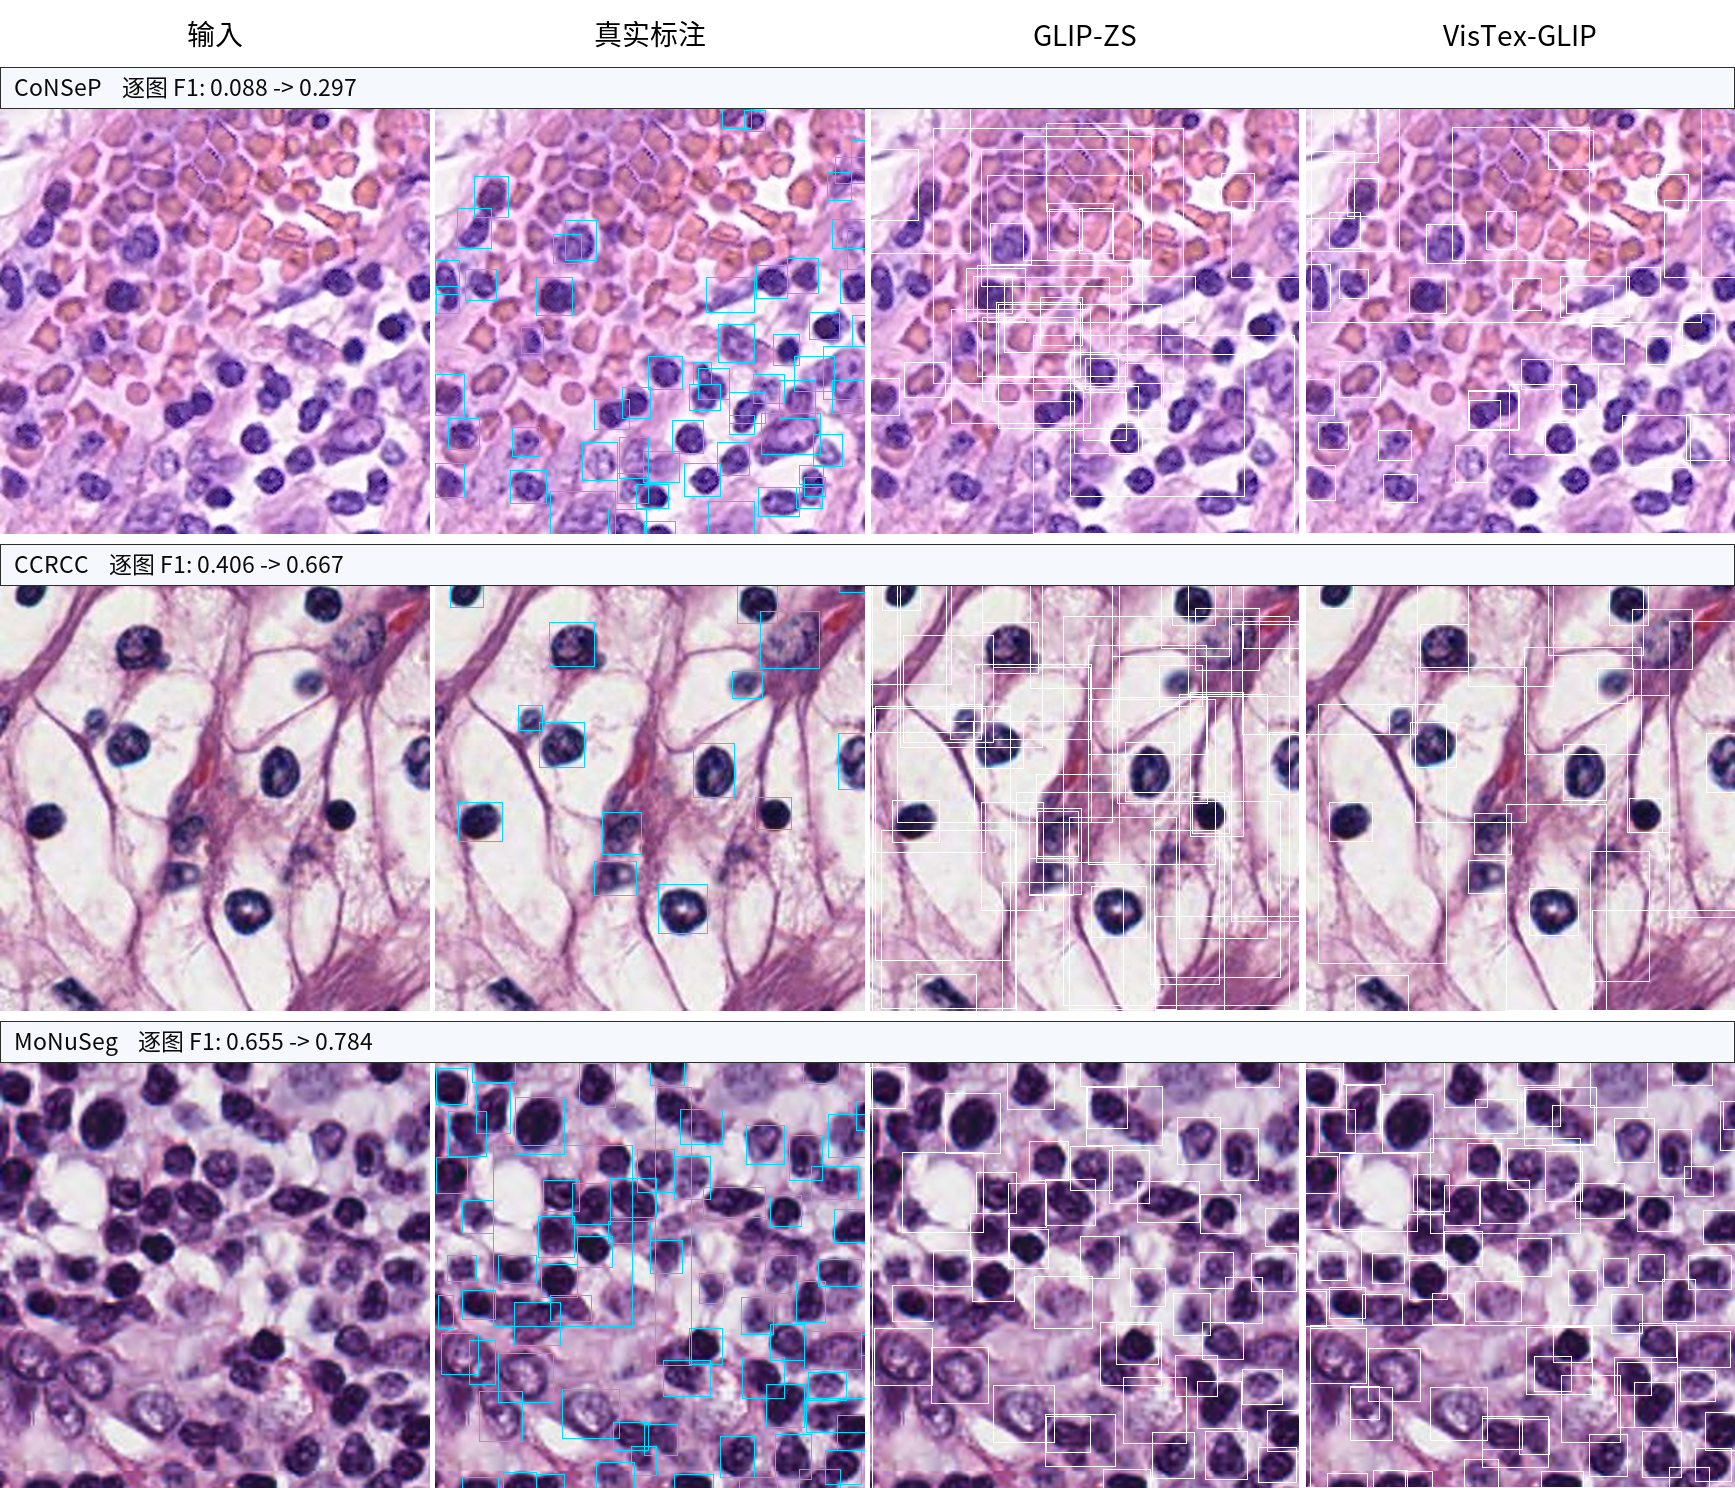
\includegraphics[width=\linewidth]{figures/figure4_3_medical_glip_vistex_ccrcc29_20260823.png}
  \caption{医学开放集检测结果可视化}
  \label{fig:vistex_medical}
\end{figure}
图~\ref{fig:vistex_medical} 从上至下给出 CoNSeP、CCRCC 与 MoNuSeg 三个病理数据集的代表性样本，从左至右依次为输入图像、真实标注、GLIP-ZS 直接预测和 VisTex-GLIP 预测。按 IoU 阈值 0.5 对所展示单图进行匹配后，F1 分别由 $0.088$ 提高至 $0.297$、由 $0.406$ 提高至 $0.667$、由 $0.655$ 提高至 $0.784$。这些逐图指标仅用于辅助解释图中漏检与定位改善，不替代数据集级总体评价。


\subsection{医学域支持图像提示的增益与消融}
为进一步区分医学域迁移增益究竟来自类别文本，还是来自支持图像中的目标外观信息，本节在相同的 2-shot 医学迁移协议下进行一个最小消融：关闭支持图像提示时，模型仅使用类别文本；开启支持图像提示时，则在相同文本提示后追加由两张医学支持图像生成的视觉文本化 token。两种设置均保持主干模型和目标域训练协议一致，因此二者之间的差异可以直接反映支持图像提示的贡献。

表 \ref{tab:vistex_medical_prompt_ablation} 汇总了五个医学数据集上的结果。关闭支持图像提示的 GLIP-ZS 在所有数据集上均明显低于开启支持图像提示的 VisTex-GLIP；后者在 MoNuSeg、CCRCC、CoNSeP、LIDC 和 DeepLesion 上分别获得 24.7、22.7、34.4、11.9 和 11.7 个百分点的 AP 提升，平均提升 21.1 个百分点。CoNSeP 上的增益最大，说明在细胞形态相近、类别边界依赖局部纹理的病理任务中，视觉支持信息能够补充单纯类别名称难以表达的形态线索。LIDC 与 DeepLesion 的增益相对较小，但方向仍保持一致，说明视觉文本化对不同医学成像风格具有一定的迁移稳定性。

需要强调的是，表 \ref{tab:vistex_medical_prompt_ablation} 与后文的当前代码复测表采用不同版本的实验协议：前者用于复现论文中的医学域提示消融，后者用于检查当前冻结推理分支在现有数据划分上的绝对表现。因此，本章不将两张表中的绝对数值直接混合排序，而是分别讨论支持图像提示带来的相对变化和当前实现的复测结果。

\begin{table}[t]
  \centering
  \caption{医学域图像提示消融}
  \label{tab:vistex_medical_prompt_ablation}
  \resizebox{\linewidth}{!}{%
  \begin{tabular}{l|rrrrr|r}
    \hline
    方法 & MoNuSeg & CCRCC & CoNSeP & LIDC & DeepLesion & 平均提升 \\
    \hline
    GLIP-ZS（关闭支持图像提示） & 4.2 & 8.8 & 1.3 & 0.3 & 0.0 & -- \\
    VisTex-GLIP（开启支持图像提示） & 28.9 & 31.5 & 35.7 & 12.2 & 11.7 & -- \\
    支持图像提示增益 & +24.7 & +22.7 & +34.4 & +11.9 & +11.7 & +21.1 \\
    \hline
  \end{tabular}}
\end{table}
表~\ref{tab:vistex_medical_prompt_ablation} 中，关闭提示时仅使用类别文本，开启提示时追加视觉文本化 token。


\subsection{关键组件消融}
表 \ref{tab:vistex_components} 将文本提示、图像提示、MSTB 参数共享和 MSF 逐项加入。只使用图像提示而移除文本提示时，新类 AP 明显下降，表明文本提供稳定的类别语义锚点；加入文本提示后，视觉 token 才能作为类内外观补充发挥作用。进一步引入 MSTB 参数共享和 MSF 后，nAP 从 41.2 提升到 51.8，说明多尺度与多阶段信息均是视觉文本化成立的关键，而不是简单地把一张支持图像编码后拼接到文本序列。

\begin{table}[t]
  \centering
  \caption{VisTex 关键组件消融}
  \label{tab:vistex_components}
  \resizebox{\linewidth}{!}{
  \begin{tabular}{l|cccc|r|rrr}
    \hline
    方法 & 文本提示 & 图像提示 & MSTB共享 & MSF & 参数量/M & AP & bAP & nAP \\ \hline
    GLIP-ZS & $\checkmark$ & $\times$ & $\times$ & $\times$ & 0.00 & 42.9 & 44.9 & 40.5 \\
    GLIP-FF & $\checkmark$ & $\checkmark^{*}$ & $\times$ & $\times$ & 397.59 & 44.3 & 44.1 & 44.7 \\
    MQ-Det & $\checkmark$ & $\checkmark$ & $\times$ & $\times$ & 53.10 & 44.7 & 43.5 & 46.3 \\ \hline
    VisTex-GLIP & $\times$ & $\checkmark$ & $\times$ & $\times$ & 38.52 & 30.6 & 32.5 & 25.9 \\
    VisTex-GLIP & $\checkmark$ & $\checkmark$ & $\times$ & $\times$ & 38.52 & 37.1 & 29.7 & 41.2 \\
    VisTex-GLIP & $\checkmark$ & $\checkmark$ & $\checkmark$ & $\times$ & 29.20 & 48.3 & 45.7 & 49.0 \\
    \textbf{VisTex-GLIP} & $\checkmark$ & $\checkmark$ & $\checkmark$ & $\checkmark$ & 63.06 & \textbf{50.3} & \textbf{48.6} & \textbf{51.8} \\ \hline
  \end{tabular}}
\end{table}
表~\ref{tab:vistex_components} 中，参数量仅统计可训练参数；$\checkmark^{*}$ 表示通过微调模型权重间接使用支持图像。


\begin{figure}[t]
  \centering
  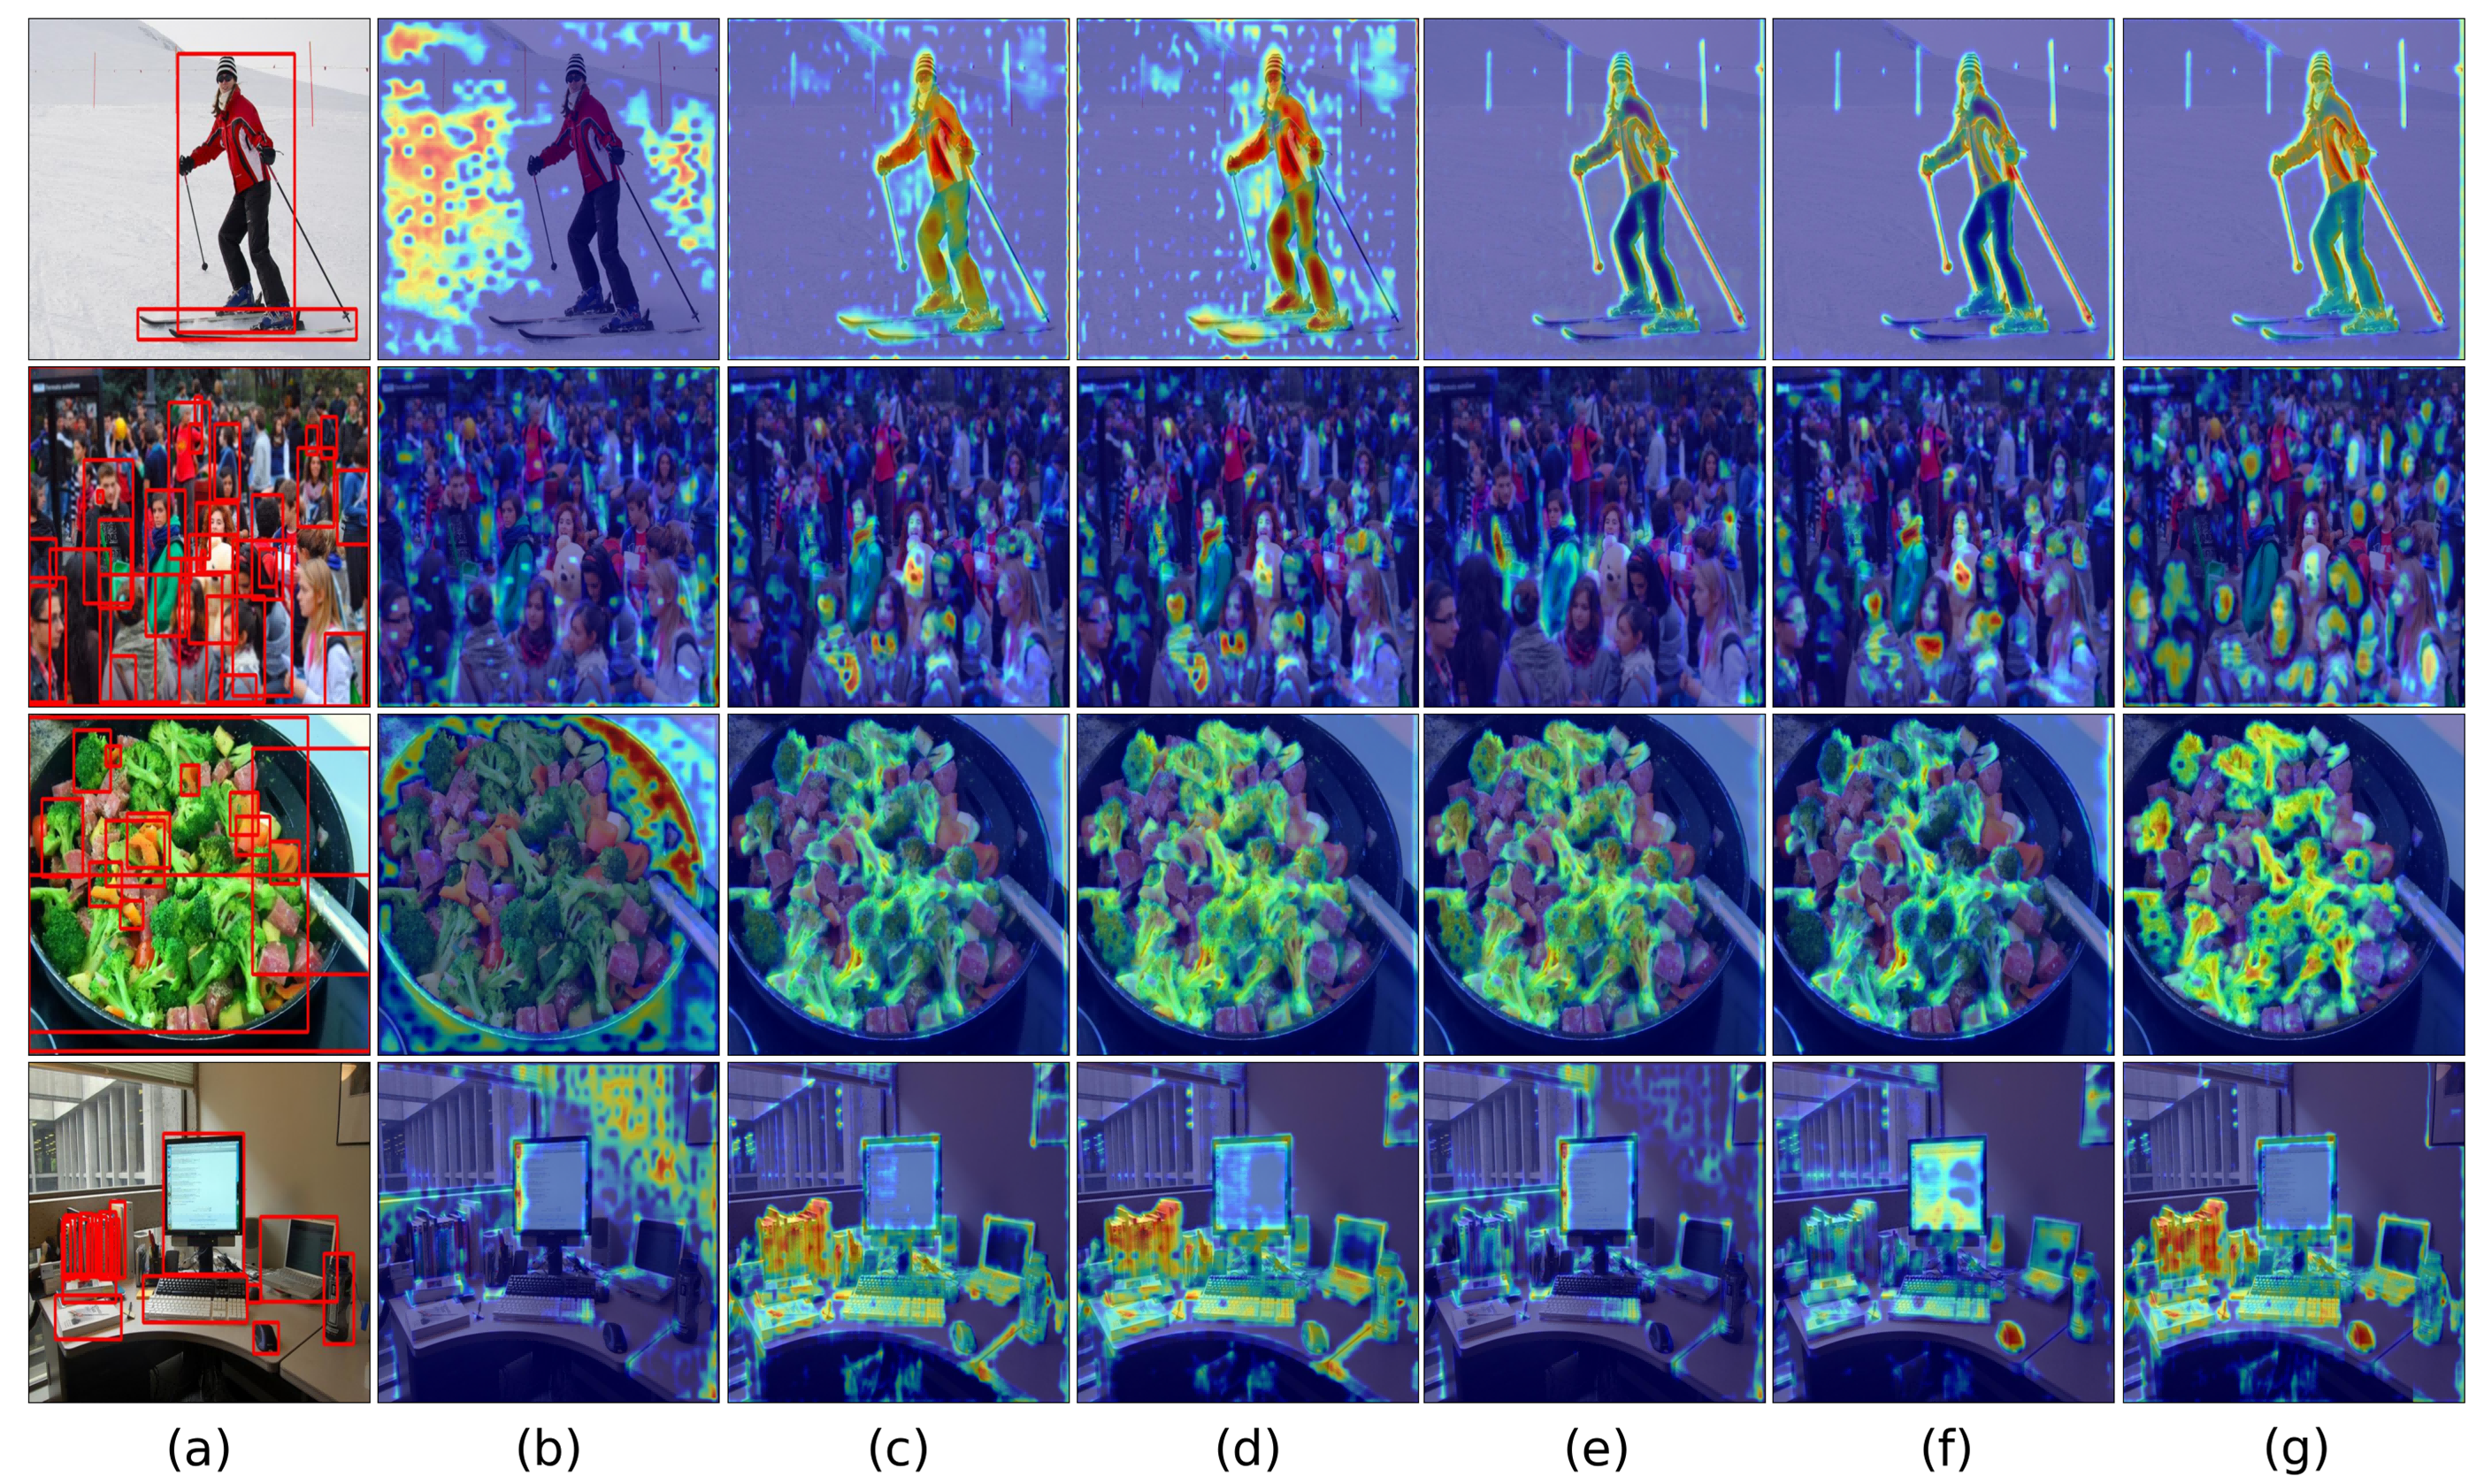
\includegraphics[width=\linewidth]{chapters/PAPERS/VisTex_ICCV_ver/corr_attentionmap.png}
  \caption{图像提示注意力响应}
  \label{fig:vistex_attention}
\end{figure}
图~\ref{fig:vistex_attention} 中，方法名及 GLIP、MQ-Det、VisTex-GLIP 等模型缩写保留英文；热区显示在文本提示基础上加入视觉文本化 token 后，查询特征对目标区域的响应更集中。


图 \ref{fig:vistex_attention} 从特征响应角度补充了定量结论。完全微调或只进行文本调节时，注意力容易扩散到背景或同类干扰区域；VisTex-GLIP 同时使用文本提示和视觉文本化 token 后，对目标轮廓及判别性局部的响应更加稳定。这说明视觉文本化并非替代语言语义，而是在保持类别语义锚点的前提下补充支持实例的外观信息。

\subsection{定性结果与失败模式}
图 \ref{fig:vistex_vis} 展示了 COCO 上与多种代表方法的输出对比。VisTex-GLIP 对小目标、遮挡目标和外观变化较大的新类具有更高召回率，同时减少了把语义相近背景误判为目标的情况。仍需指出，若支持样本本身包含严重遮挡、错误框或不具有代表性的背景，视觉 token 也可能携带偏置信息；当新类与基类在形态上高度相近时，仅依靠少量支持样本仍可能出现类别混淆。因此，支持样本质量控制与 shot 间信息融合仍是后续需要进一步研究的问题。

\begin{figure}[t]
  \centering
  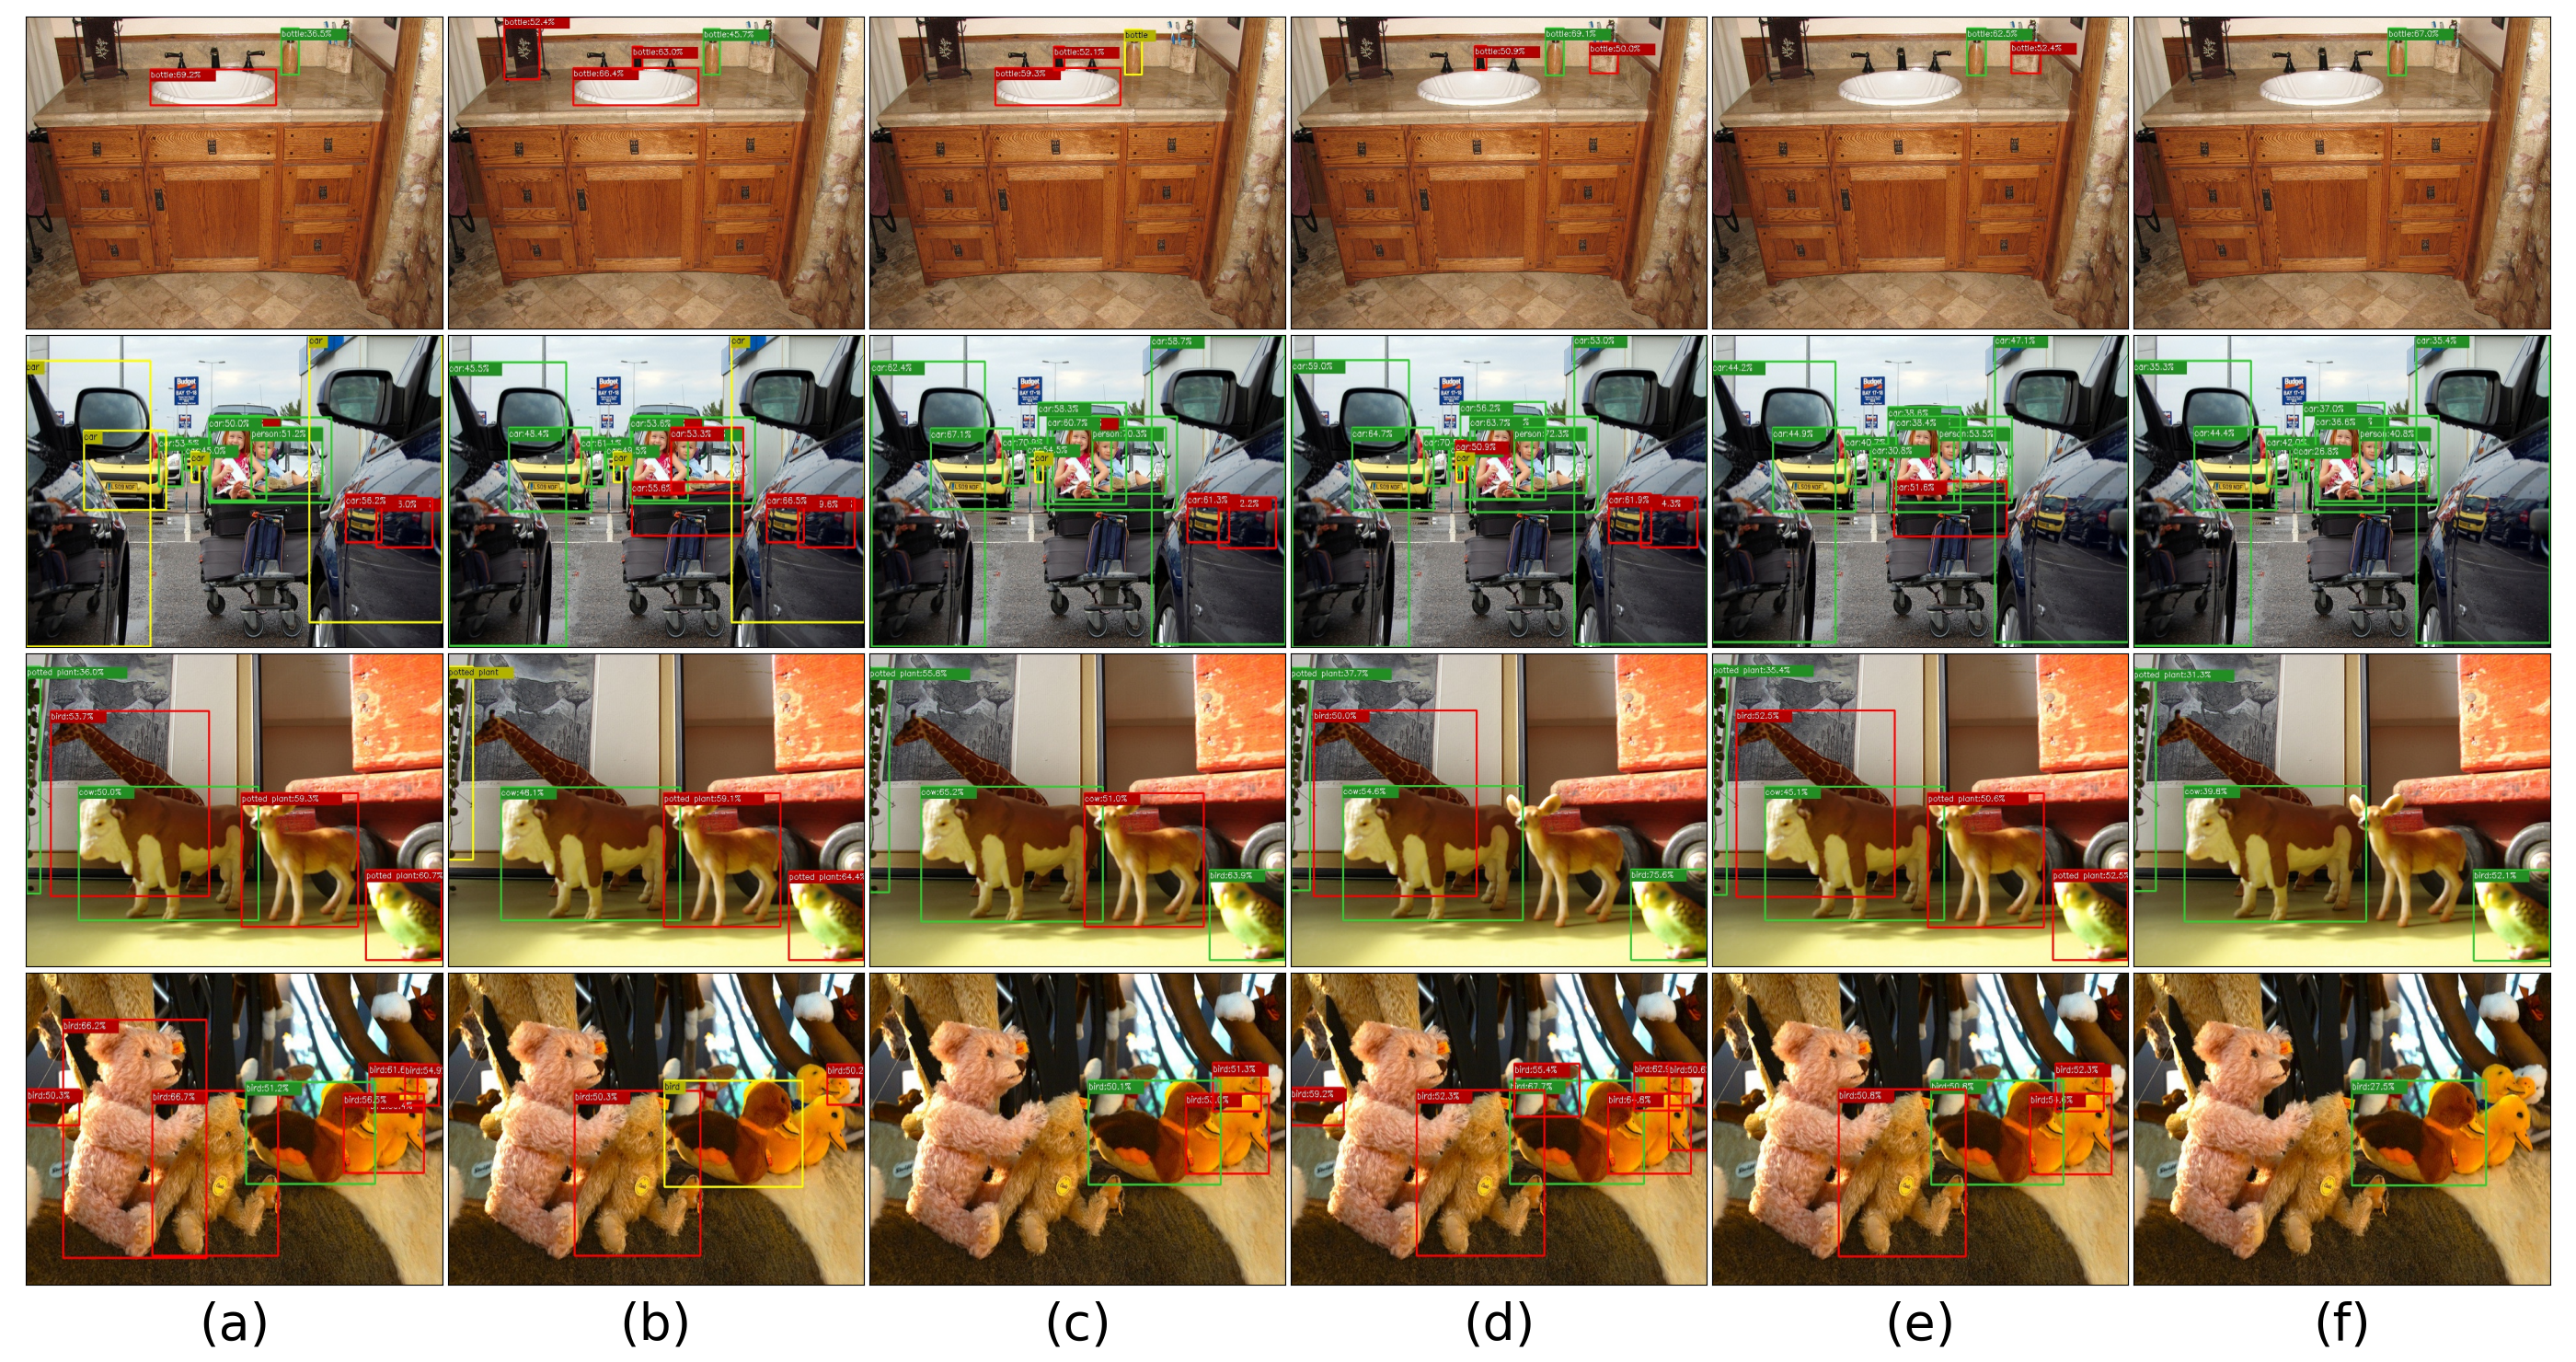
\includegraphics[width=\linewidth]{chapters/PAPERS/VisTex_ICCV_ver/vis_com.png}
  \caption{MSCOCO 检测结果可视化}
  \label{fig:vistex_vis}
\end{figure}
图~\ref{fig:vistex_vis} 中，绿/红/黄框分别表示真阳性/假阳性/假阴性。




\subsection{开放集补充结果与失败分析}
前文已经给出 MSCOCO、GFSOD、医学数据迁移和关键组件消融的原生表格。本节补充 PASCAL VOC、开放集转移及失败案例，以使视觉文本化方法的适用边界更加清楚。VisTex 的关键思想是把支持图像映射为文本特征空间中的视觉 token，而不是在 novel 类上直接改写主干参数，因此补充实验重点观察支持图像质量、尺度信息和开放集域差异。

\begin{figure}[!htbp]
  \centering
  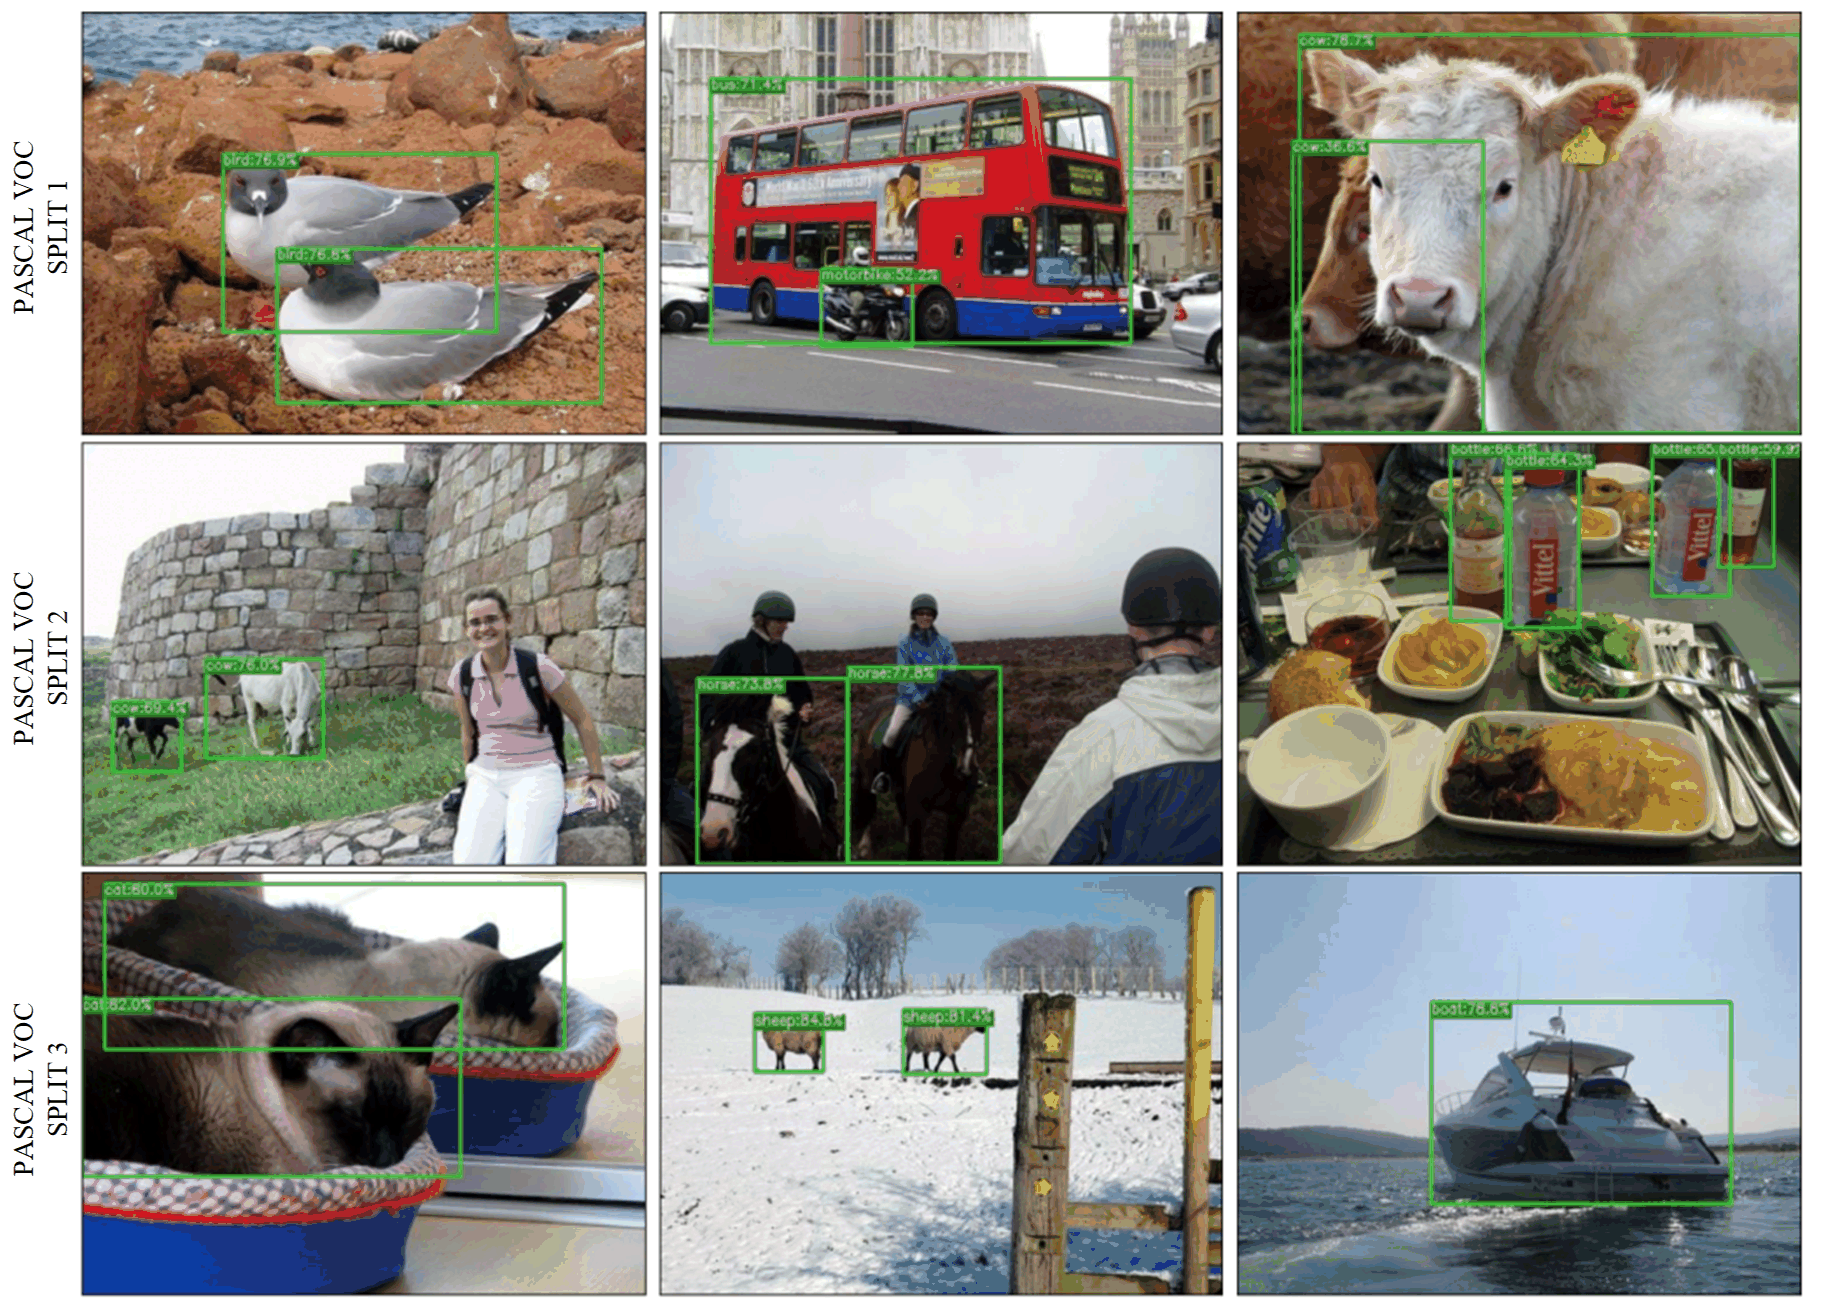
\includegraphics[width=0.78\textwidth]{chapters/PAPERS/VisTex_ICCV_ver/PASCAL VOC.png}
  \caption{PASCAL VOC 少样本检测结果}
  \label{fig:vistex_pascal}
\end{figure}
图~\ref{fig:vistex_pascal} 中，比较不同 novel split 和 shot 设置下的 AP50，说明视觉文本化不仅在 MSCOCO 上有效，也能迁移至类别划分不同的经典少样本检测基准。


\begin{figure}[!htbp]
  \centering
  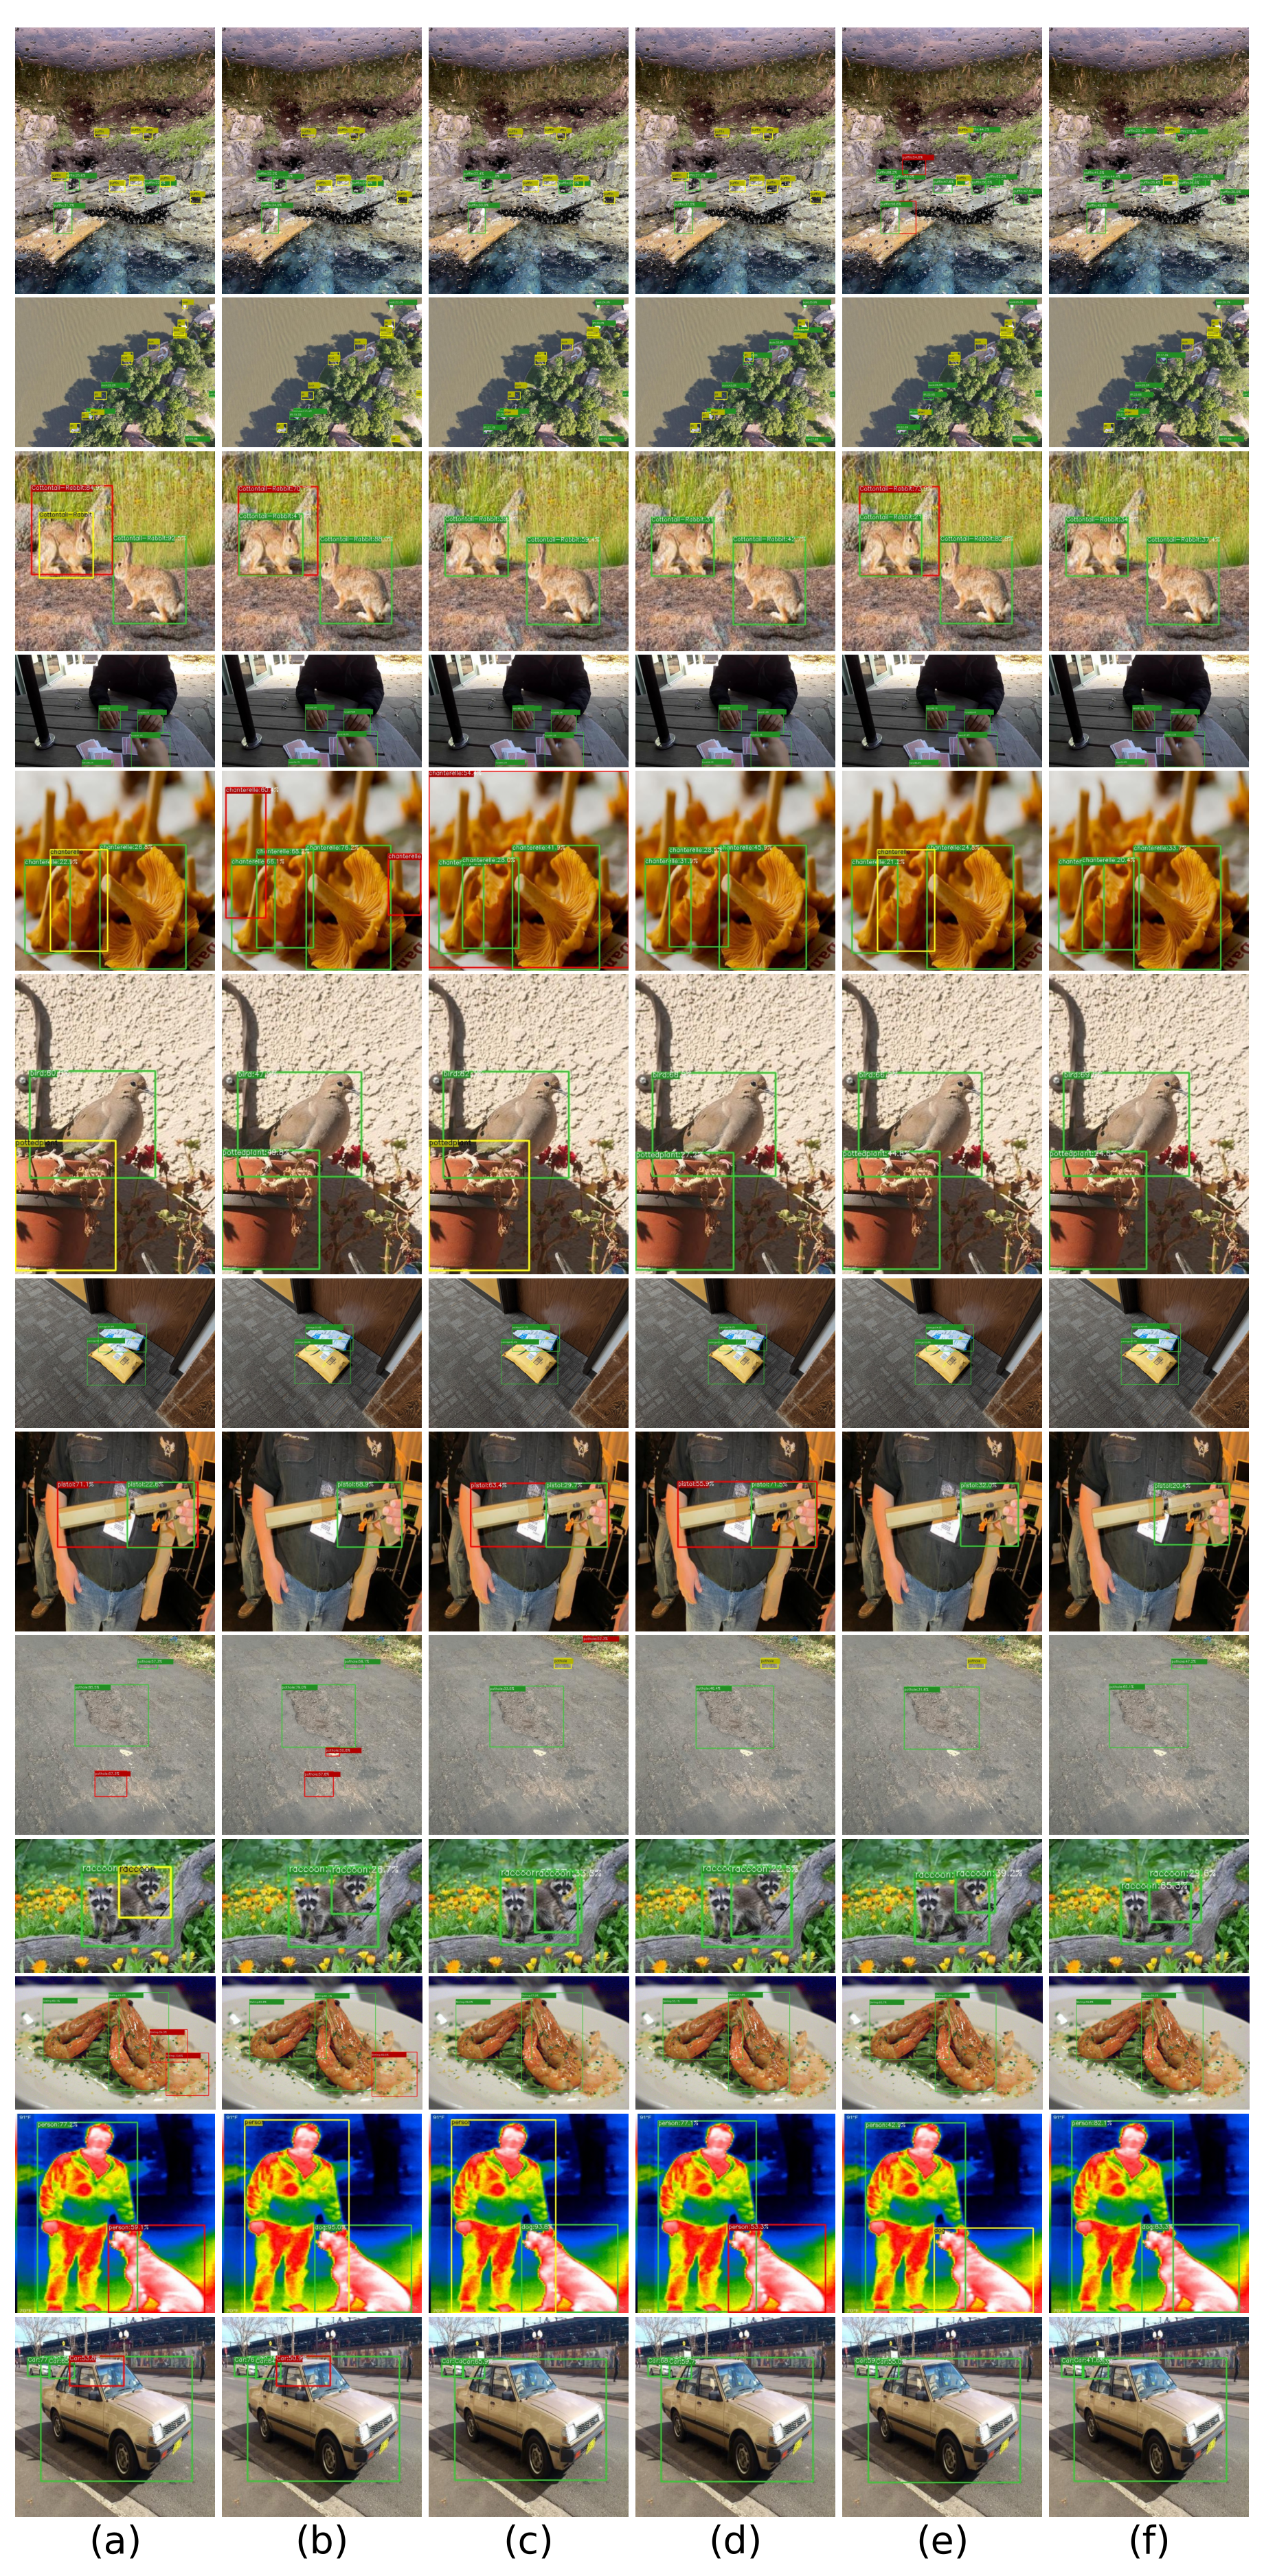
\includegraphics[width=0.58\textwidth]{chapters/PAPERS/VisTex_ICCV_ver/ODinW13_sd.png}
  \caption{ODinW13 开放集迁移结果}
  \label{fig:vistex_odinw}
\end{figure}
图~\ref{fig:vistex_odinw} 汇总了多个专业场景上的开放集迁移结果。与标准自然图像基准相比，这些数据在目标尺度、成像方式和背景结构上具有更明显的域偏移，单独依赖类别名称难以准确描述目标外观。引入少量支持图像后，VisTex 能够把颜色、局部纹理和典型轮廓编码到视觉 token 中，因此在多数子数据集上获得更稳定的检测增益。不同数据集之间的提升幅度并不完全一致，说明支持样本的代表性仍会影响视觉提示质量；图中数据集名称和方法缩写作为实验设置保留英文。


\begin{figure}[!htbp]
  \centering
  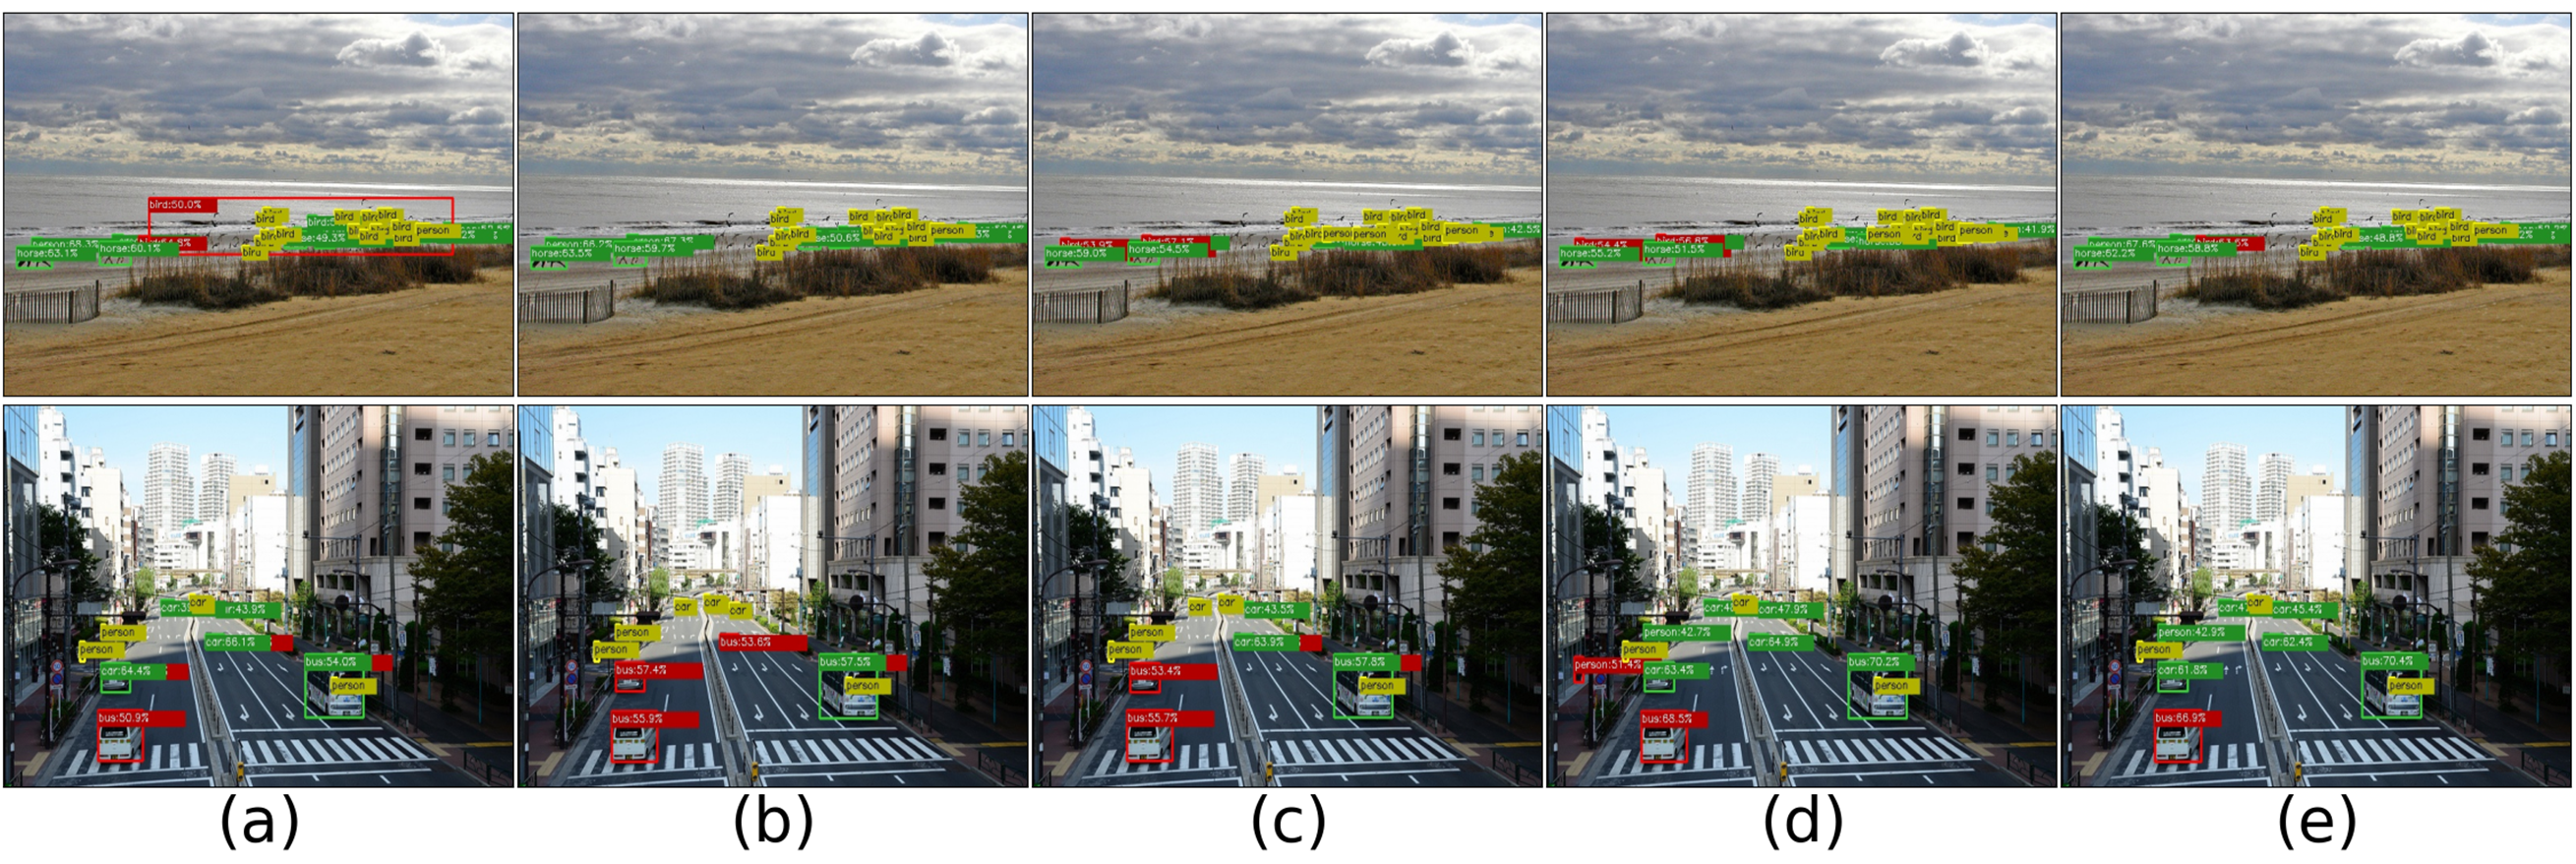
\includegraphics[width=0.76\textwidth]{chapters/PAPERS/VisTex_ICCV_ver/failure.png}
  \caption{VisTex-OVLM 典型失败案例}
  \label{fig:vistex_failure}
\end{figure}
图~\ref{fig:vistex_failure} 中，支持图像包含遮挡、背景干扰或类别外观代表性不足时，视觉 token 可能把错误背景信息带入提示序列；当 novel 类与 base 类形态高度相似时，也可能出现类别混淆。


这些补充案例说明，视觉文本化并不是无条件地解决少样本检测问题。它的优势依赖支持图像是否覆盖目标的尺度、姿态和外观变化。因此，实验报告中应同时记录支持图像的选择规则、shot 数和随机种子，而不能只报告一个未说明抽样过程的最高分。

\subsection{病理图像实例特征分布分析}
为进一步观察视觉文本化对病理图像实例表征的影响，本文在 CoNSeP 验证集上对同一批实例分别提取 GLIP-ZS 与 VisTex-GLIP 的实例级特征，并使用相同的降维参数进行 t-SNE 可视化。类别包括炎性细胞、正常上皮细胞、异型或恶性上皮细胞、成纤维细胞、肌细胞和内皮细胞等。

\begin{figure}[H]
  \centering  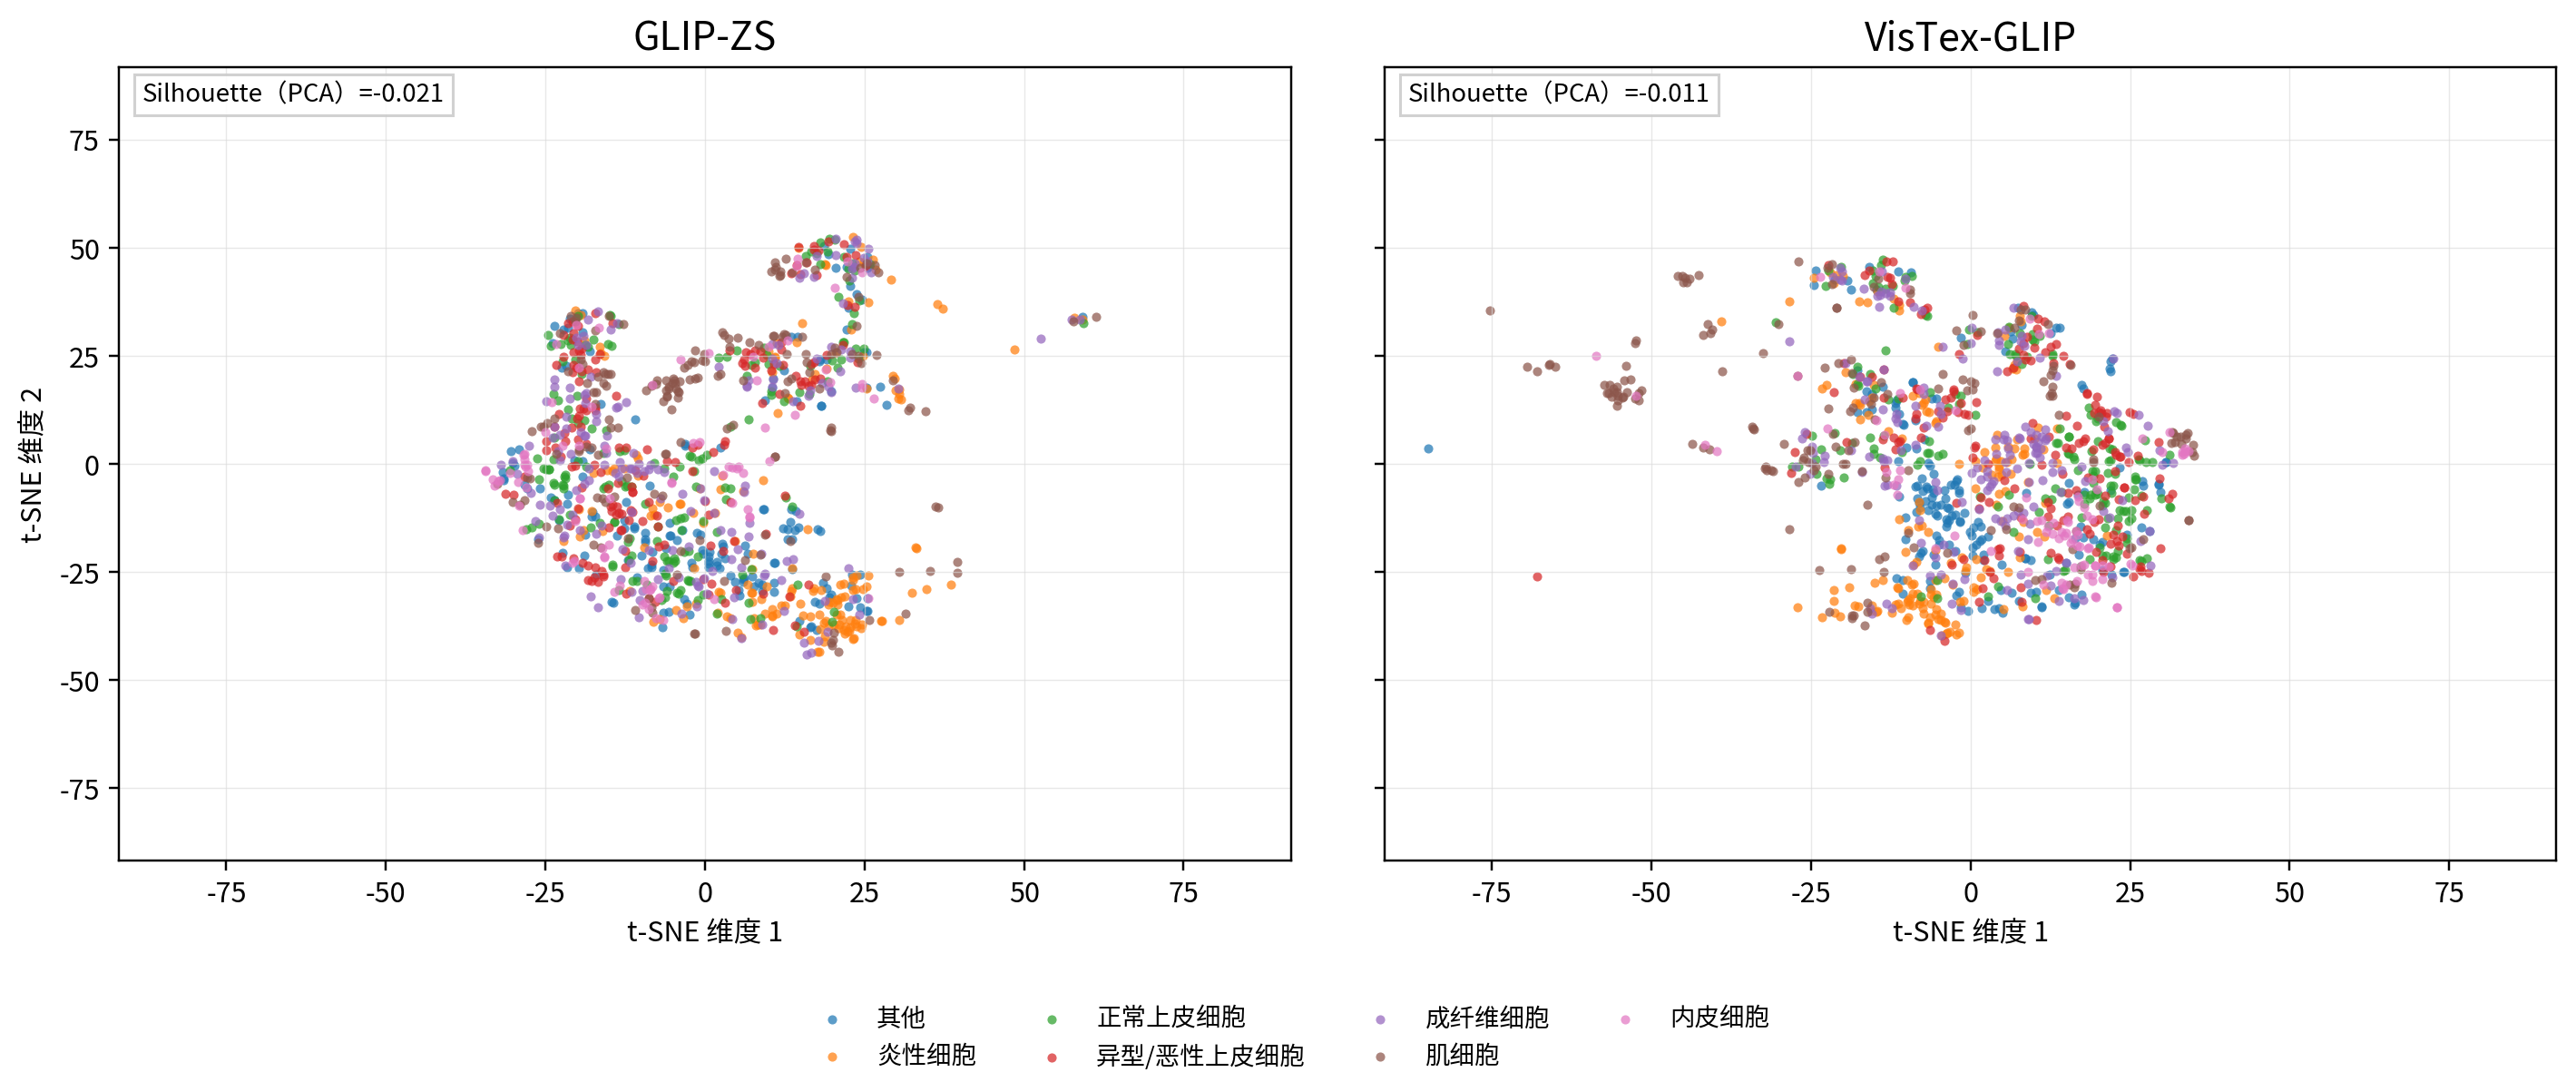
\includegraphics[width=0.96\textwidth]{figures/figure4_consep_tsne_centered_20260823.png}  \caption{GLIP-ZS 与 VisTex-GLIP 的 CoNSeP 实例特征分布}  \label{fig:vistex_consep_tsne}
\end{figure}
图~\ref{fig:vistex_consep_tsne} 中，VisTex-GLIP 的同类实例呈现更集中的趋势，PCA 特征上的轮廓系数由 $-0.021$ 提高至 $-0.011$，t-SNE 平面上的轮廓系数由 $-0.095$ 提高至 $-0.080$。这一改善幅度有限，但与检测实验中视觉提示能够补充细粒度外观线索的结论一致。为便于版面比较，左右子图仅进行了二维坐标平移居中；该显示调整不改变样本间距离、类别关系或上述评价指标。

\section{讨论}
视觉文本化的收益依赖支持样本是否覆盖目标的尺度、姿态、染色和局部上下文变化。若支持样本包含错误框、严重遮挡或非代表性背景，视觉 token 也可能把偏差写入提示序列；当新类与基类形态高度相似时，少量支持图像仍不足以完全消除类别混淆。因此，部署时应固定并报告支持集抽样规则、shot 数与随机种子，同时结合置信度校准和支持样本质量筛选。

\section{本章小结}
本章提出 VisTex-OVLM，通过视觉文本化将支持图像投影到 OVLM 的文本特征空间，使图像提示能够在不改动 OVLM 主体结构的情况下参与提示推理。借助 MSTB 的多尺度映射与 MSF 的多阶段融合，VisTex-OVLM 在标准少样本基准与开放集迁移设置中均取得了显著提升，验证了“以图像补充文本语义、且保持预训练图文对齐”的有效性。
